\documentclass[10pt,a4paper]{article}
\usepackage{amsmath}
\usepackage{graphicx}
%\usepackage{amsfonts}
%\usepackage{amssymb}
%\usepackage{eepic}
%\usepackage{babel}
\usepackage{a4wide}
\usepackage[latin1]{inputenc}
\usepackage[T1]{fontenc}

\newcounter{theproblem}
\newcommand{\problem}[1]{\addtocounter{theproblem}1\noindent {\bf Ongelma \arabic{theproblem}.}\hspace{1em}#1\bigskip

}

\addtolength{\topmargin}{-0.5cm}
\addtolength{\textheight}{1cm}

\title{Baltian Way 2008}
%\author{English}
%\subtitle{English}
%\date{Gda\'nsk, November 8, 2008}
%\linetwo{Line two}

%\version{Finnish}
%\maintitle{Baltian tie 2007}
%\linetwo{K\"o\"openhamina, 3. marraskuuta 2007}

\begin{document}
\begin{flushright}
\includegraphics[width=.25\textwidth]{MathComp2008_b}
\end{flushright}

%\maketitle

\vspace{-3em}
\begin{center}
\Huge Baltian tie 2008\bigskip

\normalsize Gda\'nsk, 8. marraskuuta 2008\smallskip

Finnish
\end{center}
Sallittu aika: 4,5 tuntia.\newline
Jokainen ongelma on 5 pisteen arvoinen.\vspace{3em}


\problem{M\"a\"arit\"a kaikki reaalikertoimiset polynomit $p(x)$, joilla
\[
p\left(\left(x+1\right)^3\right)=\left(p(x)+1\right)^3
\]
ja $p(0)=0$.}

\problem{Osoita, ett\"a jos reaaliluvut $a$, $b$ ja $c$ toteuttavat yht\"al\"on $a^2+b^2+c^2=3$, niin
\[
\frac{a^2}{2+b+c^2}+\frac{b^2}{2+c+a^2}+\frac{c^2}{2+a+b^2}\geq \frac{\left(a+b+c\right)^2}{12}.
\] 
Milloin yht\"asuuruus p\"atee?}

\problem{Onko olemassa sellainen kulma $\alpha \in \left]0,\pi/2\right[$, ett\"a $\sin\alpha$, $\cos\alpha$, $\tan \alpha$ ja $\cot \alpha$ ovat jossakin j\"arjestyksess\"a aritmeettisen jonon per\"akk\"aisi\"a termej\"a?}

\problem{ Polynomin $P$ kertoimet ovat kokonaislukuja, ja  $P(x)=5$ viidell\"a eri kokonaisluvulla~$x$. Osoita, ettei mill\"a\"an kokonaisluvulla $x$ voi olla $-6\leq P(x)\leq 4$ tai $6\leq P(x)\leq 16$.}

\problem{ Romeolla ja Julialla on kummallakin s\"a\"ann\"ollinen tetraedri, joiden kussakin k\"arjess\"a on positiivinen reaaliluku. He liitt\"av\"at jokaiseen s\"arm\"a\"an sen kahden k\"arjen lukujen tulon. Sitten he kirjoittavat jokaiselle tahkolle sen kolmen s\"arm\"an lukujen summan. Romeon tetraedrin tahkoille kirjoitetut nelj\"a lukua osoittautuvat samoiksi kuin Julian tetraedrin tahkoille kirjoitetut nelj\"a lukua. Seuraako t\"ast\"a, ett\"a Romeon tetraedrin k\"arkien nelj\"a lukua ovat samat kuin Julian tetraedrin k\"arkien nelj\"a lukua?}

\problem{ Etsi kaikki \"a\"arelliset positiivisten kokonaislukujen joukot, joissa on v\"ahint\"a\"an kaksi alkiota ja jotka toteuttavat seuraavan ehdon: jos kaksi lukua $a$ ja $b$ ($a>b$) kuuluvat joukkoon, niin my\"os $\frac{b^2}{a-b}$ kuuluu joukkoon.}

\problem{ Kuinka moni positiivisten kokonaislukujen pari $(m,n)$, jossa $m<n$, toteuttaa yht\"al\"on
\[
  \frac{3}{2008}=\frac{1}{m}+\frac{1}{n}\ ?
\]}

\problem{ Tarkastellaan positiivisten kokonaislukujen joukkoa $A$, jonka pienin alkio on $1001$ ja jonka kaikkien alkioiden tulo on kokonaisluvun neli\"o. Mik\"a on pienin mahdollinen joukon $A$ suurimman alkion arvo?}

\problem{ Positiiviset kokonaisluvut $a$ ja $b$ toteuttavat yht\"al\"on
\[
a^b-b^a=1008.
\]
Osoita, ett\"a $a$ ja $b$ ovat kongruentteja kesken\"a\"an modulo $1008$.}

\problem{ Olkoon $S(n)$ positiivisen kokonaisluvun $n$ numeroiden summa. M\"a\"arit\"a lausekkeen $\displaystyle\frac{S(n)}{S(16n)}$ suurin mahdollinen arvo.}

\problem{ Tarkastellaan joukon $\{1,2,\dots,169\}$ osajoukkoa $A$, jossa on $84$ alkiota ja jonka mink\"a\"an kahden alkion summa ei ole $169$. Osoita, ett\"a $A$ sis\"alt\"a\"a kokonaisluvun neli\"on.}


\problem{ Koululuokalla on $3n$ lasta. Jokaiset kaksi lasta tekev\"at yhteisen lahjan t\"asm\"alleen yhdelle muulle lapselle. Osoita, ett\"a kaikilla parittomilla $n$ seuraava tilanne on mahdollinen: jokaisella kolmen lapsen $A$, $B$ ja $C$ ryhm\"all\"a p\"atee, ett\"a jos $A$ ja $B$ tekev\"at lahjan $C$:lle, niin $A$ ja $C$ tekev\"at lahjan $B$:lle.}


\problem{ Tulevaa kansainv\"alist\"a matematiikkakilpailua varten osallistujamaita pyydettiin valitsemaan yhdeks\"ast\"a kombinatoriikan ongelmasta omat suosikit kilpailuteht\"aviksi. Ottaen huomioon kuinka hankalaa yksimielisyyteen p\"a\"aseminen yleens\"a on, kukaan ei ollut yll\"attynyt, kun k\"avi n\"ain:
\begin{itemize}
\item Jokainen maa \"a\"anesti t\"asm\"alleen kolmea teht\"av\"a\"a.
\item Jokaiset kaksi maata \"a\"anestiv\"at eri teht\"av\"ajoukkoja.
\item Mill\"a tahansa kolmella maalla on jokin teht\"av\"a, jota mik\"a\"an maista ei \"a\"anest\"anyt.
\end{itemize}
Mik\"a on suurin mahdollinen osallistujamaiden lukum\"a\"ar\"a?}

\problem{Onko mahdollista rakentaa $4\times 4\times 4$ -kuutio kuvan mukaisista, nelj\"ast\"a yksikk\"okuutiosta koostuvista palikoista?}

\begin{center}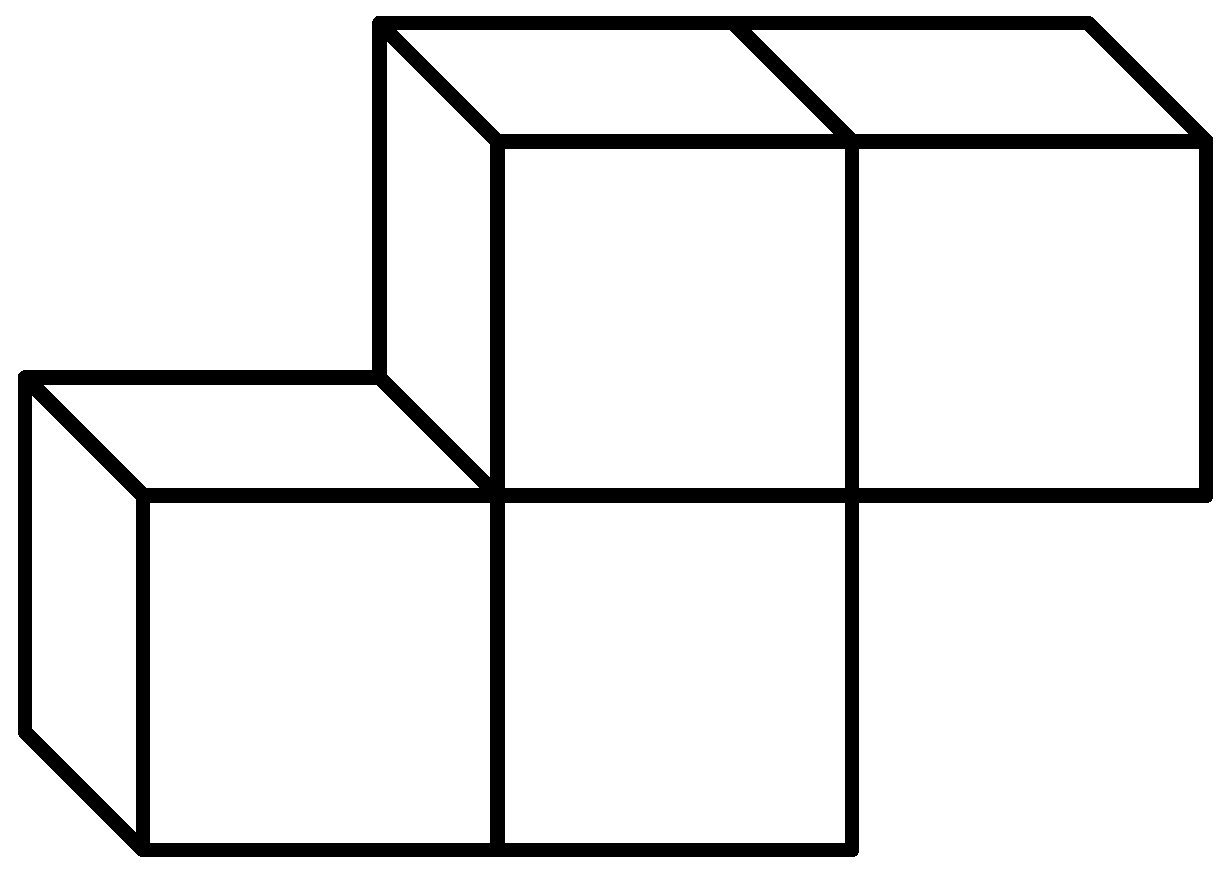
\includegraphics[width=.15\textwidth]{tetris}\end{center}


\problem{ $n\times n$ -ruudukolle asetetaan kaksi vierekk\"aist\"a ruutua peitt\"avi\"a $1\times 2$ -dominoita siten, ett\"a ne eiv\"at koske toisiinsa (edes kulmissa) ja ett\"a niiden peitt\"am\"a ala on $2008$. Etsi pienin $n$, jolla t\"am\"a onnistuu.}

\problem{ Olkoon $ABCD$ suunnikas. Ympyr\"a, jonka halkaisija on $AC$, leikkaa suoran $BD$ pisteiss\"a $P$ ja $Q$. Pisteen $C$ kautta piirretty suoran $AC$ kohtisuora leikkaa suorat $AB$ ja $AD$ pisteiss\"a $X$ ja $Y$. Osoita, ett\"a pisteet $P$, $Q$, $X$ ja $Y$ ovat samalla ympyr\"all\"a.}

\problem{ Olkoot $a$, $b$, $c$ ja $d$ annetun ympyr\"an sis\"a\"an piirretyn nelikulmion sivut. Osoita, ett\"a tulo $\left(ab+cd\right)\left(ac+bd\right)\left(ad+bc\right)$ saavuttaa maksiminsa kun nelikulmio on neli\"o.}

\problem{ Olkoon $AB$ ympyr\"an $S$ halkaisija ja $L$ pisteeseen $A$ piirretty tangentti. Olkoon lis\"aksi $c$ kiinnitetty positiivinen reaaliluku. Tarkastellaan kaikkia suoran $L$ pistepareja $X$ ja $Y$, jotka sijaitsevat pisteen $A$ eri puolilla, niin ett\"a $|AX|\cdot |AY|=c$. Suorat $BX$ ja $BY$ leikkaavat ympyr\"an $S$ pisteiss\"a $P$ ja $Q$. Osoita, ett\"a kaikki t\"allaiset suorat $PQ$ kulkevat yhteisen pisteen kautta.}

\problem{ Ykk\"oshalkaisijaisen ympyr\"an sis\"a\"an piirret\"a\"an j\"anteit\"a. Niiden pituuksien summa on yli $19$. Osoita, ett\"a ympyr\"all\"a on halkaisija, joka leikkaa ainakin seitsem\"a\"a j\"annett\"a.}

\problem{Olkoon piste $M$ janalla $BC$ ja piste $N$ janalla $AB$, niin ett\"a $AM$ ja $CN$ ovat kolmion $ABC$ kulmanpuolittajia. Lis\"aksi
\begin{equation*}
  \frac{\angle BNM}{\angle MNC}=\frac{\angle BMN}{\angle NMA}.
\end{equation*}
Osoita, ett\"a kolmio $ABC$ on tasakylkinen.}

\end{document}
